\chapter{Foundations of Multi-Agent Reinforcement Learning}

\section*{Introduction}
Multi-agent reinforcement learning (MARL) is, in essence, reinforcement learning (RL) applied to multi-agent game models to learn optimal policies for the agents. Thus, MARL is deeply rooted in both RL theory and game theory. This chapter provides the necessary theoretical background, starting with the foundational principles of single-agent RL before extending them to the multi-agent domain.

\section{Single-Agent Reinforcement Learning}
To understand how multiple agents learn and interact, we must first understand how a single agent learns. This section introduces the theory and algorithms of RL when there is only a single agent for which we want to learn an optimal policy. We will begin by providing a general definition of RL, following which we will introduce the Markov decision process (MDP) as the foundational model used in RL to represent single-agent decision processes. Based on the MDP model, we will define basic concepts such as expected returns, optimal policies, value functions, and Bellman equations. Most of the MARL algorithms introduced later in this chapter build on these concepts and essentially extend them to multi-agent game models.
\begin{figure}[h!]
    \centering
    % This is a placeholder for your figure. 
     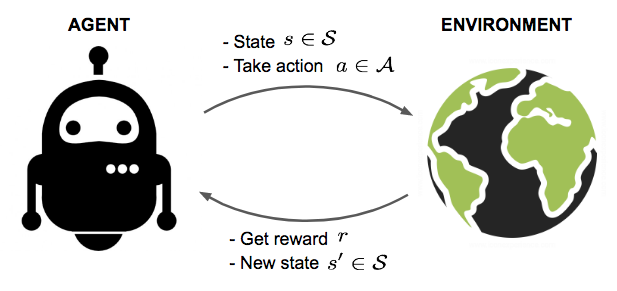
\includegraphics[width=0.48\textwidth]{img_pfe/RL_illustration.png}
    % \fbox{\rule{0pt}{4in} \rule{0.9\linewidth}{0pt}} 
    \caption{An agent interacts with the environment, trying to take smart actions to maximize cumulative rewards.}
    \label{fig:rl}
\end{figure}

\subsection*{General Definition of Reinforcement Learning}
We begin by providing a general definition of reinforcement learning:
\begin{quote}
    \textit{Reinforcement learning (RL) algorithms learn solutions for sequential decision processes via repeated interaction with an environment.} 
\end{quote}
This definition raises three main questions:
\begin{enumerate}
    \item What is a sequential decision process?
    \item What is a solution to the process?
    \item What is learning via repeated interaction?
\end{enumerate}

A sequential decision process is defined by an agent that makes decisions over multiple time steps within an environment to achieve a specified goal. In each time step, the agent receives an observation from the environment and chooses an action. Given the chosen action, the environment may change its state according to some transition dynamics and send a scalar reward signal to the agent. This fundamental interaction is often visualized as the RL loop.
\begin{figure}[h!]
\centering

 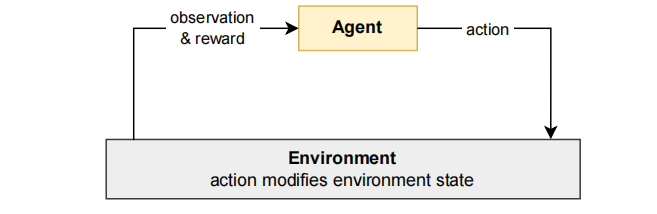
\includegraphics[width=0.8\textwidth]{img_pfe/rl_loop.PNG}
\caption{Basic reinforcement learning loop for a single-agent system.}
\label{fig:rl_loop}
\end{figure}



A solution to the decision process is an optimal decision policy for the agent, which chooses actions in each state to achieve some specified learning objective. Typically, the learning objective is to maximize the expected return for the agent in each possible state. The return is defined as the sum of rewards received over time.

Finally, RL algorithms learn via repeated interaction by trying different actions in different states and observing the outcomes. This method is often described as “trial and error.” A central problem in this learning process is the exploration-exploitation dilemma: how to balance exploring the outcomes of different actions versus sticking with (exploiting) actions that are currently believed to be best.

RL is a distinct type of machine learning. It is not supervised learning, because reward signals do not directly tell the agent which action to take. It also differs from unsupervised learning because the rewards, while not a supervised signal, act as feedback from which to learn an optimal policy. In the following sections, we will formally define these concepts within the framework of the Markov decision process.

\subsection*{Markov Decision Processes (MDPs)}
The standard model used in RL to formalize the sequential decision process is the Markov decision process.

\begin{definition}[Markov decision process]
A finite Markov decision process (MDP) consists of:
\begin{itemize}
    \item A finite set of states $\mathcal{S}$
    \item A finite set of actions $\mathcal{A}$
    \item A reward function $R: \mathcal{S} \times \mathcal{A} \times\mathcal{S} \rightarrow \mathbb{R}$
    \item A state transition probability function $T: \mathcal{S} \times \mathcal{A} \times \mathcal{S} \rightarrow [0,1]$
    \item An initial state distribution $\mu: \mathcal{S} \rightarrow [0,1]$
\end{itemize}
\end{definition}

At each time step $t$, the agent observes the current state $s_t \in \mathcal{S}$ and chooses an action $a_t \in \mathcal{A}$ according to its policy, $\pi(a_t | s_t)$. The MDP then transitions to a next state $s_{t+1}$ with probability $T(s_{t+1} | s_t, a_t)$, and the agent receives a reward $r_t = R(s_t, a_t, s_{t+1})$. This process continues until a terminal state is reached.

The term “Markov” comes from the Markov property, which states that the future is conditionally independent of the past, given the present state and action:
$$
\Pr(s_{t+1}, r_t | s_t, a_t, s_{t-1}, a_{t-1}, \dots, s_0, a_0) = \Pr(s_{t+1}, r_t | s_t, a_t)
$$

This means the current state provides all necessary information to make an optimal decision. The most common assumption in RL is that the dynamics of the MDP (the transition and reward functions) are a priori unknown to the agent.

An important special case of the MDP is the Partially Observable Markov Decision Process (POMDP), where the agent receives an observation $o_t$ rather than the true state $s_t$. POMDPs are a special case of the multi-agent models we will introduce later.

\subsection{Dynamic programming}
There are two basic families of algorithms to compute optimal policies for MDPs: dynamic programming and temporal-difference learning.
Dynamic programming requires complete knowledge of the MDP specification
and uses this knowledge to compute optimal value functions and policies. In
contrast, temporal-difference learning does not require complete knowledge
of the MDP, instead, it learns optimal value functions and policies by inter-
acting with the environment and generating experiences.

\subsubsection{Policy Iteration}

Policy iteration is an iterative algorithm used to compute the optimal policy for a Markov Decision Process (MDP). It consists of two main steps: policy evaluation and policy improvement.

1. \textbf{Policy Evaluation}: Given a policy \(\pi\), we evaluate its value function \(V^\pi(s)\) by solving the following system of linear equations for all states \(s \in \mathcal{S}\):

\[
V^\pi(s) = \sum_{a \in \mathcal{A}} \pi(a|s) \sum_{s' \in \mathcal{S}} P(s'|s, a) \left[ R(s, a, s') + \gamma V^\pi(s') \right]
\]

where:
\begin{itemize}
    \item \(\pi(a|s)\) is the probability of taking action \(a\) in state \(s\) under policy \(\pi\),
    \item \(P(s'|s, a)\) is the transition probability from state \(s\) to state \(s'\) given action \(a\),
    \item \(R(s, a, s')\) is the reward received when transitioning from state \(s\) to state \(s'\) given action \(a\),
    \item \(\gamma\) is the discount factor.
\end{itemize}

2. \textbf{Policy Improvement}: Using the value function \(V^\pi(s)\) computed in the policy evaluation step, we improve the policy by choosing actions that maximize the expected value. The improved policy \(\pi'\) is given by:

\[
\pi'(s) = \arg\max_{a \in \mathcal{A}} \sum_{s' \in \mathcal{S}} P(s'|s, a) \left[ R(s, a, s') + \gamma V^\pi(s') \right]
\]

The policy iteration algorithm alternates between these two steps until the policy converges to the optimal policy \(\pi^*\).

\subsubsection{Value Iteration}

Value iteration is another dynamic programming algorithm used to find the optimal policy by iteratively updating the value function. Unlike policy iteration, value iteration combines policy evaluation and policy improvement into a single step. The Bellman equation for value iteration is given by:

\[
V_{k+1}(s) = \max_{a \in \mathcal{A}} \sum_{s' \in \mathcal{S}} P(s'|s, a) \left[ R(s, a, s') + \gamma V_k(s') \right]
\]

where \(V_k(s)\) is the value function at iteration \(k\).

Once the value function \(V(s)\) has converged, the optimal policy \(\pi^*\) can be extracted as:

\[
\pi^*(s) = \arg\max_{a \in \mathcal{A}} \sum_{s' \in \mathcal{S}} P(s'|s, a) \left[ R(s, a, s') + \gamma V(s') \right]
\]

Both policy iteration and value iteration are powerful methods in dynamic programming for solving MDPs and computing optimal policies. Both their algorithms can be found in the Annex. In the next section, we dig deep into the Bellman equations for states and action functions that are the foundation of the policy iteration and value iteration algorithms.




\subsection{Bellman's Optimality equations}
There are two key Bellman equations used in dynamic programming for Markov Decision Processes (MDPs): the state value function and the state-action value function. These equations provide the foundation for computing optimal policies by recursively breaking down the expected returns.


\begin{itemize}
    \item \textbf{State Value function for policy $\pi$:} The value of a state is the expected return starting from that state; depends on the agent’s policy: 
    \begin{equation}
    V^{\pi} (s) = E_{\pi} \{ R_t | s_t = s \} = E_{\pi} \{ \sum _{k=0} ^{\infty} \gamma ^{k} r_{t+k+1} | s_t=s \}
    \end{equation}
    \item \textbf{Action Value function for policy $\pi$}: The value of taking an action in a state under policy $\pi$ is the expected return starting from that state, taking that action, and thereafter following $\pi$:
    \begin{equation}
        Q^{\pi} (s,a) = E_{\pi} \{ R_t | s_t = s, a_t =a \} = E_{\pi} \{ \sum _{k=0} ^{\infty} \gamma ^{k} r_{t+k+1} | s_t=s, a_t =a \}
    \end{equation}
\end{itemize}

We can calculate the reward as: 
\begin{equation}
\begin{aligned}
     R_t = &  r_{t+1} + \gamma r_{t+2} + \gamma ^{2} r_{t+3} + \gamma ^{3} r_{t+4} + \cdots
     \\     R_t = & r_{t+1} + \gamma R_{t+1}
\end{aligned}
\end{equation}
\vspace*{0.1cm}

So the \textbf{state-value function} and the \textbf{Action-value function} become: 
\begin{equation}
\begin{aligned}
        V^{\pi} (s) = & E_{\pi} \{ R_t | s_t = s \} = E_{\pi} \{ r_{t+1} + \gamma V^{\pi} (s_{t+1}) | s_i = s \} 
        \\     Q^{\pi} (s,a) = E_{\pi} \{ R_t & | s_t = s, a_t=a \} = E_{\pi} \{ r_{t+1} + \gamma V^{\pi} (s_{t+1}) | s_i = s, a_t=a \}
\end{aligned}
\end{equation}
\vspace*{0.1cm}

In a \textbf{deterministic} environment, the state-value function and the action-value function are defined as: 

\begin{equation}
\begin{aligned}
        V^{\pi} (s) & =  r(s, \pi (s) , s') + \gamma V^{\pi} (s')
  \\           Q^{\pi} (s,a) & =  r(s, a , s') + \gamma V^{\pi} (s')
\end{aligned}
\end{equation}


The Bellman equations provide a way to decompose the problem of finding optimal policies into simpler, recursive relationships involving value functions. However, in practice, several challenges necessitate the use of estimations (approximations) rather than exact calculations. We use \textbf{TD errors }to quantify the discrepancy between the predicted and actual outcomes as computed by the Bellman equations:

\begin{equation}
    \begin{aligned}
        TDerror(s) = & \ V^{\pi} (s) - \sum _{s'} T(s, \pi (s) , s') [ r(s, \pi (s) , s') + \gamma V^{\pi} (s')]
        \\
        TDerror(s,a) = & \ Q^{\pi} (s,a) - \sum _{s'} T(s, a , s') [ r(s, a , s') + \gamma V^{\pi} (s')]
    \end{aligned}
\end{equation}

Estimating these errors helps in adjusting the value functions \( V^{\pi}(s) \) and \( Q^{\pi}(s,a) \) towards more accurate representations of the true values.


The goal is for the agent (or agents) to find the \textbf{optimal policy} $\pi ^{*}$ using the \textbf{Bellman Backup} that we will go into in the next section. Optimal policies are the greedy policies with respect to the functions $V^{*}$ or $Q^{*}$. And we say \textbf{Bellman's Optimality equations} to talk about the state-value function, as well as the action-value function in the case of learning the optimal policy $\pi ^{*}$.
\begin{figure}[H]
    \centering
    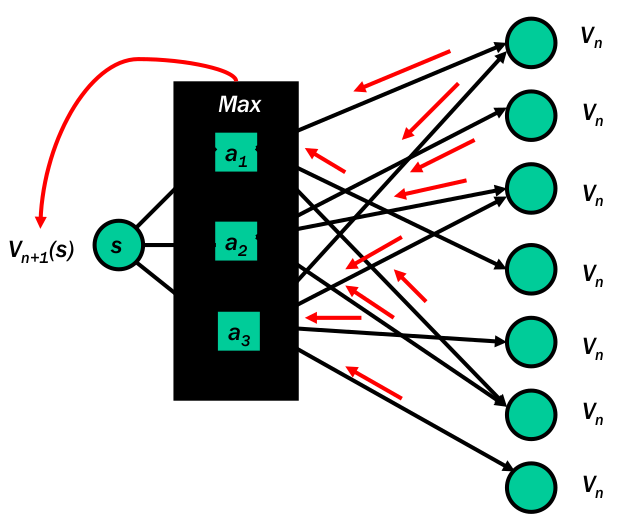
\includegraphics[width=0.5\linewidth]{images_pfe/Screenshot from 2024-06-14 17-08-41.png}
    \caption{Bellman Backup}
    \label{fig:Bellman-Backup}
\end{figure}




